\documentclass[10pt,twocolumn,letterpaper]{article}

\usepackage{cvpr}
\usepackage{times}
\usepackage{epsfig}
\usepackage{graphicx}
\usepackage{amsmath}
\usepackage{amssymb}
\usepackage{subfigure}
\usepackage{url}

\usepackage{float}
\floatstyle{boxed} 
\restylefloat{figure}

% Include other packages here, before hyperref.

% If you comment hyperref and then uncomment it, you should delete
% egpaper.aux before re-running latex.  (Or just hit 'q' on the first latex
% run, let it finish, and you should be clear).
\usepackage[breaklinks=true,bookmarks=false]{hyperref}

\cvprfinalcopy % *** Uncomment this line for the final submission

\def\cvprPaperID{****} % *** Enter the CVPR Paper ID here
\def\httilde{\mbox{\tt\raisebox{-.5ex}{\symbol{126}}}}

% Pages are numbered in submission mode, and unnumbered in camera-ready
%\ifcvprfinal\pagestyle{empty}\fi
\setcounter{page}{1}
\begin{document}

%%%%%%%%% TITLE
\title{Enhancing Low-Light Images on Mobile Devices}

\author{Jeff Chen\\
School of Computer Science\\
Carnegie Mellon University\\
{\tt\small jeffrey@cmu.edu}
% For a paper whose authors are all at the same institution,
% omit the following lines up until the closing ``}''.
% Additional authors and addresses can be added with ``\and'',
% just like the second author.
% To save space, use either the email address or home page, not both
\and
Graeme Rock\\
Robotics Institute\\
Carnegie Mellon University\\
{\tt\small grock@andrew.cmu.edu}
}

\maketitle
%\thispagestyle{empty}

%%%%%%%%% ABSTRACT
\begin{abstract}
   We propose that contrast-limited adaptive histogram equalization, or CLAHE, can be used to enhance images and video taken in low-light conditions on mobile devices. We will show that with proper optimizations, CLAHE can be used in real time on high-definition video, and that the resulting enhanced image is suitable for use in augmented-reality systems. With our optimized algorithm, we achieve over 90 frames per second on a 720p video on an iPhone 6S. We demonstrate our results with an iOS application that applies CLAHE to a live video feed.
\end{abstract}

%%%%%%%%% BODY TEXT
\section{Introduction}

Augmented reality apps are increasing in popularity as mobile SoCs and cameras grow more powerful. However, many augmented reality apps fail under poor lighting conditions. While there are ways to increase low-light fidelity at a hardware level (increasing brightness and contrast, for example), these methods are often insufficient. Instead, post-capture processing must be used to further enhance low-light imagery.

Histogram equalization (HE) is a method of increasing an image's global contrast using the image's histogram. It works well when the image's background and foreground are both bright or both dark. however, in images where there already is high global contrast (such as a mostly dark image with a single bright light), HE will not change the image much, because the global contrast is already high. HE also does not distinguish between noise and signal, so noise will often be amplified using this method. As such, HE is typically suitable for scientific images like thermal, satellite, or x-ray images.

Adaptive histogram equalization (AHE) is a method of increasing local contrast in an image. It differs from ordinary histogram equalization in that AHE computes a histogram corresponding to each pixel of the image, and uses these local histograms to redistribute the brightness values of the image. Therefore, AHE improves local contrast rather than global contrast of an image. AHE has a tendency to overamplify noise in relatively homogenous regions - a region where all the pixels differ only very slightly in intensity in the original image will become very distinctly noisy in the post-AHE image.

A variant of this algorithm, known as contrast-limited adaptive histogram equalization (CLAHE), limits the amplification. The contrast amplification for a given pixel depends on the slope of the local cumulative distribution function (CDF), and therefore depends on the value of the local histogram at that pixel value. CLAHE clips the local histogram at a predefined value before calculating the CDF, limiting the slope of the CDF and therefore the contrast amplification. The part of the histogram that is clipped is then redistributed among the other bins in the histogram. See Figure 1 for the naive CLAHE algorithm.

\begin{figure}[h]
\caption{\textbf{Naive CLAHE algorithm}}
For each pixel $p$: 
\begin{enumerate}
\itemsep0em 
\item Produce the histogram of the square of the pixels surrounding $p$. Typically, this square is 8x8 or 16x16, and the histogram has 128 or 256 bins. (Fewer than 128 bins compromises the quality of the output image.)
\item Clip the histogram at the specified limit (frequently between 2 and 4), and redistribute the excess values equally among the remaining bins. 
\item Create a mapping $M$ from input to output intensities by building a CDF (cumulative distribution function) from the histogram.
\item Set the output pixel $p' = M(p)$.
\end{enumerate}
\end{figure}

CLAHE produces high-quality enhanced images under most lighting conditions. However, implemented naively, CLAHE is unusable for real-time applications: a naive implementation of CLAHE running on 1280x720 video on an iPhone 6S took 1.6 seconds to process each frame. In this paper we show that with the proper optimizations, CLAHE is suitable for real-time video processing and therefore augmented reality apps.

\section{Background}

The original CLAHE paper \cite{Zuiderveld} provides a better-than-naive implementation of CLAHE in ANSI C. However, this implementation is still insufficiently fast for real-time video. On 720p video on an iPhone 6S, this implementation ran at about 10 frames per second. To achieve real-time performance, we would have to scale down the video resolution unacceptably.

There exist highly optimized implementations of CLAHE for MIMD (multiple-instruction-multiple-data) machines \cite{Kurak}, and for nVidia desktop GPUs \cite{Hillaire}. However, due to architectural differences, these implementations do not directly translate to iOS.

GPUImage is an open-source library that provides a set of image processing algorithms that are optimized to run on the GPU of an iOS device. GPUImage provides an algorithm for traditional HE, but does not contain a CLAHE implementation, or the primitives necessary to implement CLAHE.

ARM NEON is a general-purpose SIMD engine that efficiently processes multimedia formats. It is present on modern Apple mobile devices, including the iPhone 6 and iPhone 6S. Using SIMD to vectorize algorithms often produces significant speedups at the cost of additional code complexity.

Grand Central Dispatch (GCD) is a threadpool implementation developed by Apple that allows iOS applications to easily take advantage of thread-level parallelism. Properly architected (with respect to cache coherence and locality) image processing algorithms can take advantage of this parallelism to achieve massive speedups without significantly increasing code complexity.

\section{Approach}

Our CLAHE implementation runs approximately 145x faster than the naive implementation. The majority of this speedup is by modifying the CLAHE algorithm so that significantly fewer pixel accesses are required. We achieved more speedup by leveraging the hardware available on modern iPhones - specifically, by using NEON intrinsics and by taking advantage of the iPhone's multicore processor. Finally, we achieved some minor speedups by optimizing math operations.

\subsection{Tiling}

The naive CLAHE algorithm generates a histogram for each pixel in the image. For an $n \times m$ image with a neighborhood of $a$ pixels, this requires approximately $nma^2$ memory accesses just to build the histogram. Furthermore, these memory accesses are not ordered optimally, which will lead to cache thrashing and additional performance degradation.

Tiling the image allows for a significant improvement in efficiency without compromising the quality of the result. We partition the image into small tiles (8x8 and 16x16 tiles are common choices). We then compute the histogram, CDF, and mapping for each tile. This reduces the number of memory accesses when building the histogram to just $nm$ (64x fewer memory accesses than the naive version using 8x8 neighborhoods), since each pixel is included in only one histogram. These mappings are suitable for the center pixel of each tile. Every other pixel is transformed using up to four mapping of the tiles closest to them. Pixels in the majority of the image are bilinearly interpolated. Pixels lying close to edges are linearly interpolated, and pixels near corners use only the mapping of the corner tile.

\subsection{NEON}

Our implementation leverages NEON intrinsics to achieve faster clipping and mapping of each local histogram. We use 16-bit unsigned integers to hold histogram values, and NEON on the arm64 architecture supports 128-wide vectors. Then, any vectorized code will take one-eighth as many iterations to complete (although each iteration may take slightly longer to account for loading and storing the vectors). \footnote{We could decrease the number of iterations and runtime further by using multiple vectors in each loop and taking advantage of instruction-level parallelism. This is left as an exercise for the reader.} The basic clipping algorithm is shown in Figure 2:
\begin{figure}[h]
\caption{\textbf{Histogram clipping algorithm}}
Given a histogram $H$ with $n$ bins and clip limit $c$:
\begin{enumerate}
\itemsep0em 
\item Find the total area $a$ of the histogram above the clip limit.
\item For each bin $b$ in the histogram:
	\begin{enumerate}
	\itemsep0em 
	\item If $H(b) > c$, set $H(b) = c$.
	\item Else, if $H(b) + \frac{a}{n} > c$, set $H(b) = c$ and subtract $c - H(b)$ from $a$.
	\item Else, set $H(b) = H(b) + \frac{a}{n}$ and subtract $\frac{a}{n}$ from $a$.
	\end{enumerate}
\item Equally distribute the remaining excess into bins, ensuring that no bin goes above the clip limit.
\end{enumerate}
\end{figure}

Steps 1 and 2 of the histogram clipping algorithm can be effectively vectorized using NEON intrinsics. Our implementation can be found in the functions \verb"get_excess()" and \verb"clip_histogram()" in \verb"clahe_neon.cpp". 

Our implementation also uses NEON to map each local histogram. The mapping algorithm simply produces a CDF out of the histogram. This is exactly the prefix sum problem. The well known parallel solution for this problem does not work on NEON, as it is intended for massively parallel architectures like GPUs. Instead, we implemented a different algorithm, that reduces the number of operations per histogram from 256 additions to 96 vector operations. The vectorized code also takes advantage of instruction-level parallelism, further increasing the speed. Our algorithm is given in Figure 3.
\begin{figure}[h]
\caption{\textbf{A vectorized algorithm for prefix-sum}}
Given an array $A$ of size $n$ (assuming 16-bit integers and 128-wide vectors):
\begin{enumerate}
\itemsep0em
\item For each 8-element subarray $v$ of the array in parallel:
	\begin{enumerate}
	\itemsep0em
	\item Set $v = v + \verb"rshift"(v, 1)$
	\item Set $v = v + \verb"rshift"(v, 2)$
	\item Set $v = v + \verb"rshift"(v, 4)$
	\end{enumerate}
Now, every $v$ contains the eight-element prefix sum starting at $v(0)$. 
\item Set $i$ to an 8-wide vector, filled with $0$.
\item For each 8-element subarray $v$ of the array:
	\begin{enumerate}
	\itemsep0em
	\item Set $v = v + i$
	\item Set $i$ to an 8-wide vector, filled with $v(7)$.
	\end{enumerate}
\end{enumerate}
\end{figure}

Our implementation of prefix-sum in NEON can be found in \verb"map_histogram()" in \verb"clahe_neon.cpp". \footnote{This implementation is not quite pure prefix-sum. It also multiplies every element in the histogram by a scalar to support proper mapping of input to output intensities.}

\subsection{Grand Central Dispatch}
We use Grand Central Dispatch (GCD) to further improve performance of our algorithm. Specifically, the \verb"dispatch_apply()" function acts like a parallel loop. Crucially, the function only exits when every task in the loop completes. We use \verb"dispatch_apply()" three separate times inside our implementation. First, we parallelize histogram generation. To maximize cache efficiency, each task handles a single row of histograms (and therefore 8 rows of the image). When this task has completed, we also parallelize histogram clipping and mapping. Each task handles one histogram's tiling and mapping, since mapping must occur after tiling. Finally, we parallelize the interpolation process, again with each task handling a single tile (or 64 pixels).

\subsection{Other Speedups}

We were able to obtain numerous smaller speedups by using the following techniques:
\begin{itemize}
\itemsep0em
\item Using 16-bit instead of 32-bit unsigned integers for histograms.
\item Infrequently allocating and deallocating memory.
\item Taking advantage of locality when iterating through the input image.
\item Approximating floating-point math with fixed-point math wherever possible.
\item Limiting the tile size and histogram bin count to powers of 2, allowing us to use bitshifts instead of divisions and multiplications.
\item We can also greatly increase performance by shrinking the number of bins in a histogram. This also degrades the quality of the image.
\end{itemize}

\section{Results}

We built an app that allows a user to toggle CLAHE, HE, as well as color and interpolation. See Figure \ref{fig:table} and Figure \ref{fig:doorway} for some screenshots of our application in action. Looking more thoroughly at the screenshots, we see that CLAHE offers superior results to both no filter and HE in Figure \ref{fig:table}. With no filter, the table is totally invisible. With HE, although the table is visible, it is overwhelmed by noise. In Figure \ref{fig:doorway}, we compare CLAHE with interpolation and without interpolation. In the interpolation-less image, one can see artifacts generated by tiling the histograms: the pixels at each side of a tile border are amplified differently. However, in the interpolated image, these artifacts are greatly reduced. We could reduce the artifacts further by using larger tile sizes.

As stated in the introduction, we achieved a 145x speedup over the naive implementation. On a grayscale 720 video feed on an iPhone 6S, we can run CLAHE with interpolation at over 90FPS (11ms per image). With tiling as our only optimization, we achieve about 10FPS, or 100ms per image. Much of the remaining speedup come from vectorization and parallelization. See Figure \ref{fig:perf} for a logarithmic graph of the performance we achieve on a 720p grayscale image on an iPhone 6S.

\begin{figure}[h]
\caption{\textbf{Performance of various optimizations for CLAHE. Metrics are on an iPhone 6S with a grayscale 1280x720 image}}
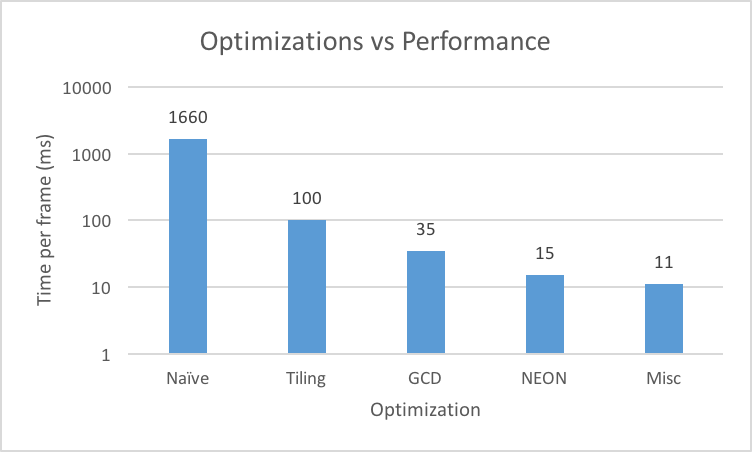
\includegraphics[width=\linewidth]{perf.png}
\label{fig:perf}
\end{figure}

When running on color images, however, we only achieve 20FPS. This is because we must first convert incoming camera image from RGB to HSL, then runs CLAHE (or HE) on the intensity values, then convert back to RGB. These conversions reduces FPS significantly. However, most applications will not require CLAHE to be run on color images.

We believe that our implementation achieved performance suitable for integration with augmented reality apps. Since we operate at 11ms per frame, an AR app using CLAHE still has 22ms to do other image processing. Also, our implementation does not use the GPU, so an AR app could simultaneously process images on the GPU while running CLAHE. 

\section{Future Work}
Future work will involve continuing to optimize CLAHE. We believe that we could further enhance performance by using OpenGL and the GPU. We would also like to build a demo augmented reality app using CLAHE. Additionally, we would like to improve the UI of our demo app to support different CLAHE options, like the clip limit, bin size, and tile size, which are currently hardcoded. 

\section{List of Work}

Graeme tested some preliminary ideas. The code used in the app and final writeup were written by Jeff.

\section{GitHub Page}

Our application and final report are available at {\tt\small https://github.com/Low-Light-AR/Low-light-AR}.

{\small
\bibliographystyle{ieee}
\bibliography{egbib}
}

\newpage

\begin{figure*}[h]
\caption{A table, with various filters enabled}
  \centering
  \subfigure[Table in color, with no filter applied]{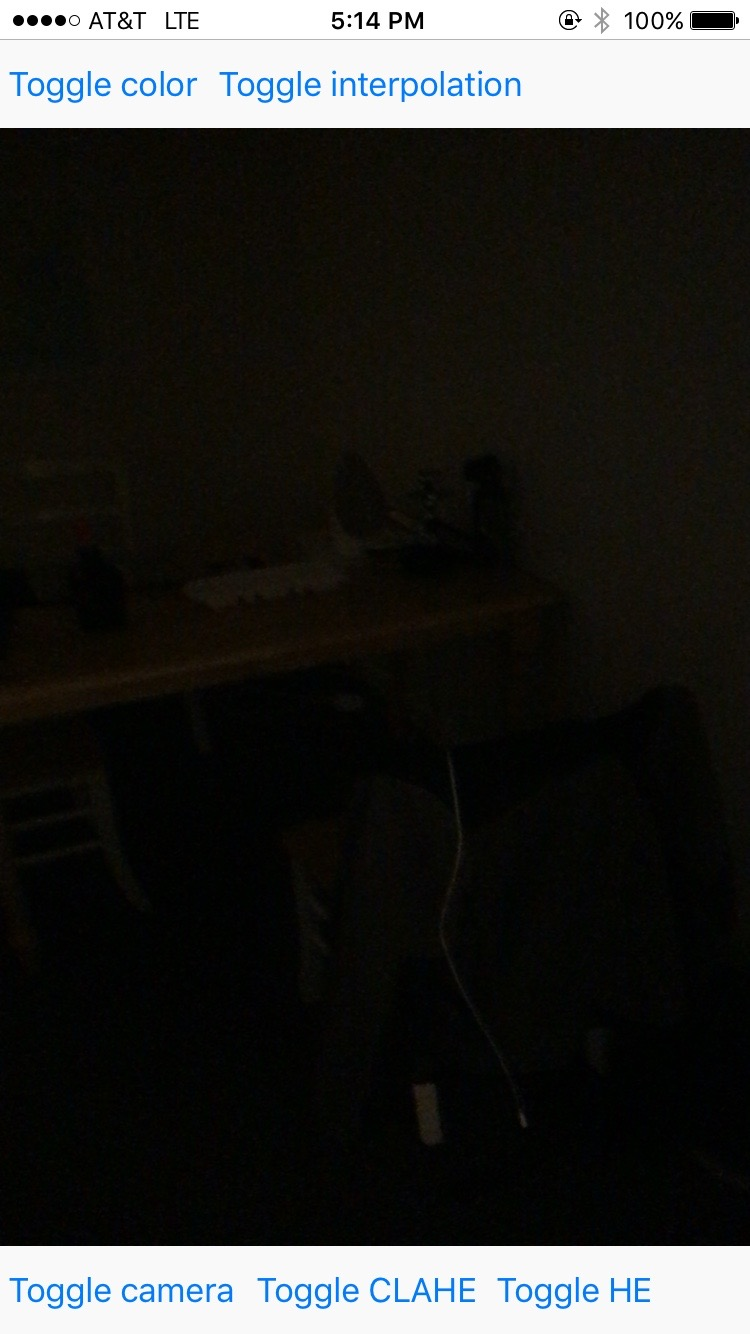
\includegraphics[width=0.33\linewidth]{table_nofilter.jpg}}\quad
  \subfigure[Table in color, with CLAHE enabled]{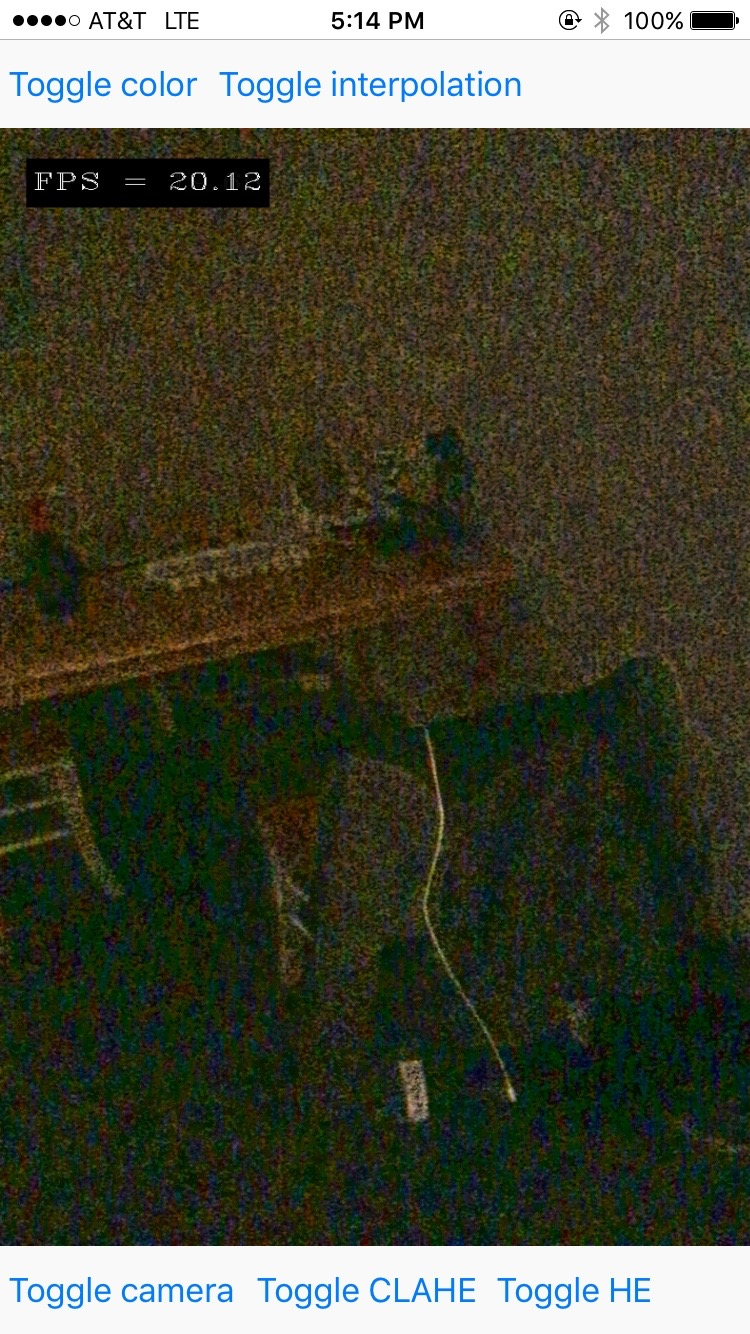
\includegraphics[width=0.33\linewidth]{table_clahe.jpg}}\quad
  \subfigure[Table in color, with HE enabled]{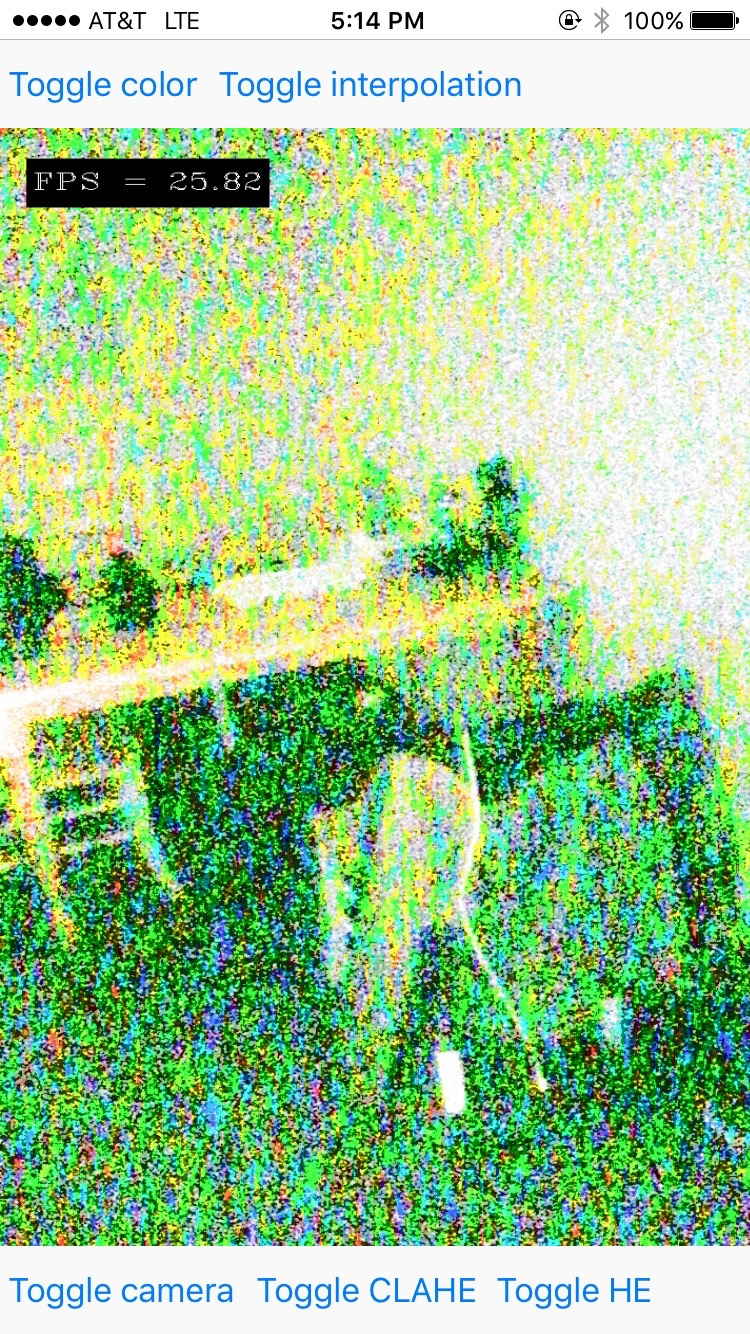
\includegraphics[width=0.33\linewidth]{table_he.jpg}}
\label{fig:table}
\end{figure*}

\begin{figure*}[h]
\caption{A doorway, with various filters enabled}
  \centering
  \subfigure[Doorway with no filter applied]{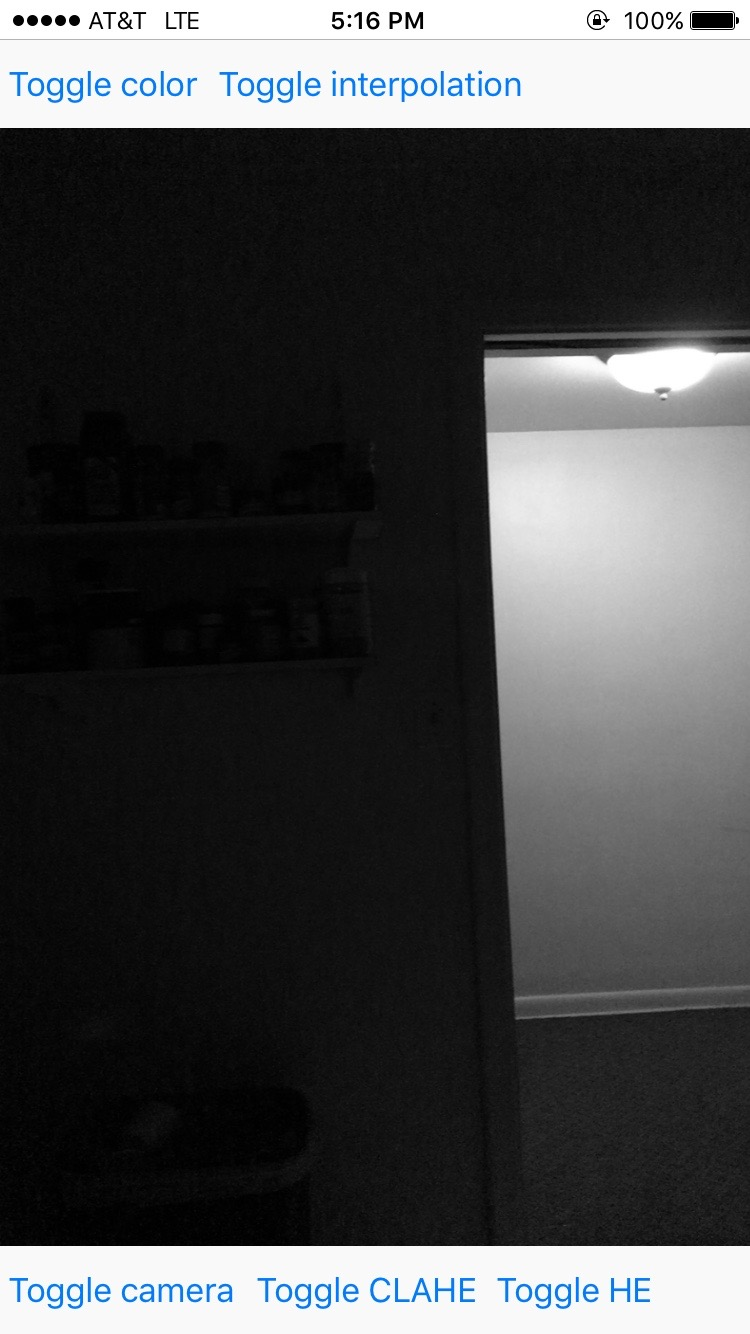
\includegraphics[width=0.33\linewidth]{doorway_nofilter.jpg}}\quad
  \subfigure[Doorway with CLAHE and interpolation]{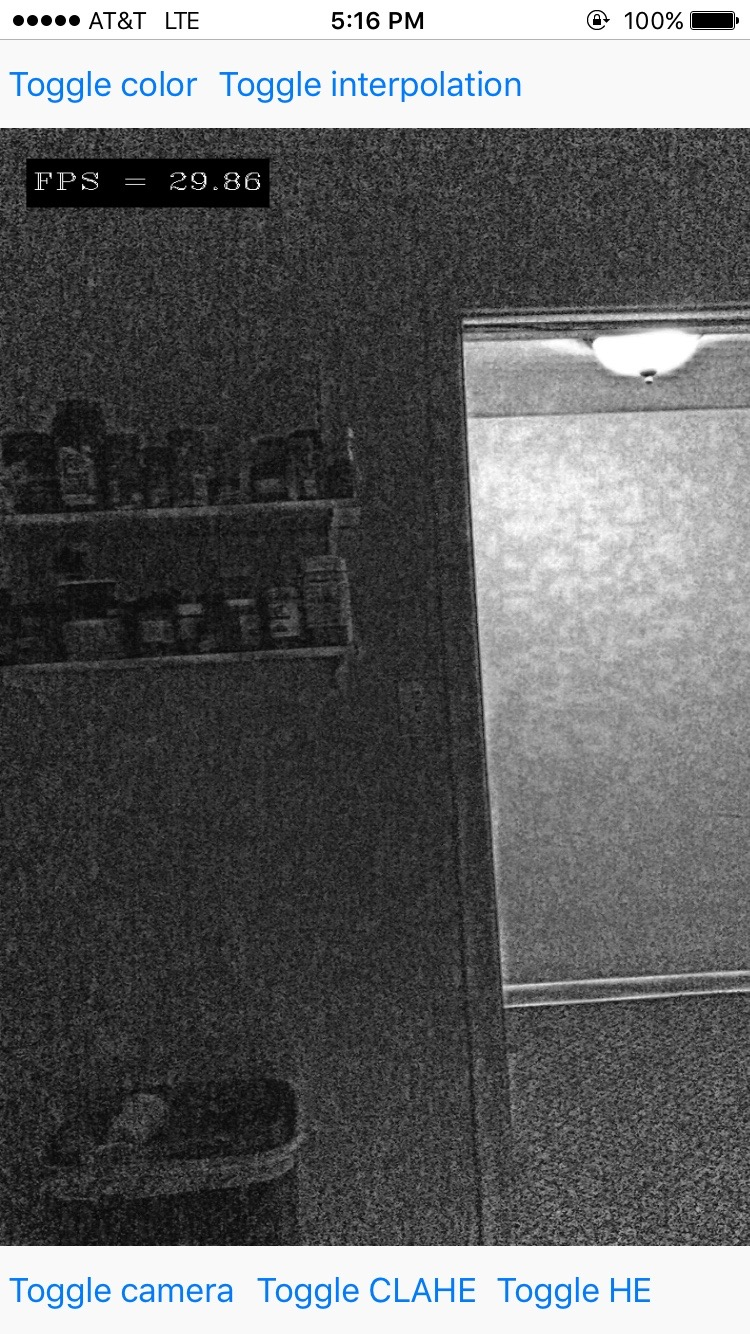
\includegraphics[width=0.33\linewidth]{doorway_interp.jpg}}\quad
  \subfigure[Doorway with CLAHE and no interpolation]{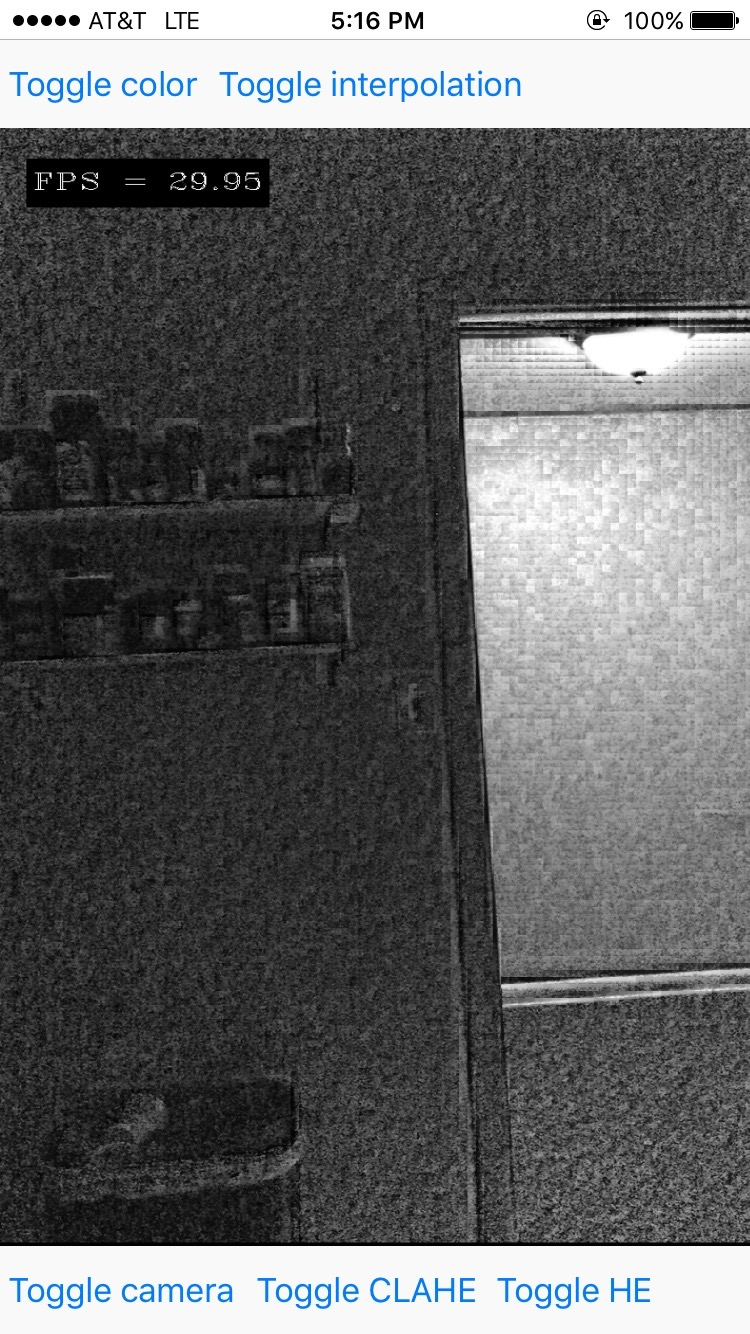
\includegraphics[width=0.33\linewidth]{doorway_nointerp.jpg}}
\label{fig:doorway}
\end{figure*}

\end{document}
